\chapter{Aktueller Stand der Performance Analyse in der \acl{CE}}
\label{sec:analyse}
In der \ac{CE} werden bereits verschiedene Wege genutzt, um die Performance und
das Verhalten der HANA Datenbank zu analysieren. 
\section{Google Benchmark}
\label{sec:google_benchmark}

Google Benchmark ist ein Open Source Benchmarking Tool von Google,
welches es einem ermöglicht einzelne Funktionen in C++ zu benchmarken. 
Dazu kann man ähnlich zu den meisten Test Frameworks drei verschiedene
Codeabschnitte definieren.

Der Hauptabschnitt definiert was genau im Benchmark untersucht werden
soll. Diese legt die für die Messung relevante Logik fest.
Der Setup Abschnitt wird einmal vor jeder Ausführung des Benchmarks
aufgerufen. In dieser werden die Voraussetzungen für die Ausführung des Hauptabschnitts
geschaffen. Man könnte sie beispielsweise nutzen, um Testdaten für den Benchmark
zu generieren oder zu laden, da er nicht bei den Messungen beachtet wird.
Der Teardown Abschnitt wird nach jeder Ausführung des Benchmarks aufgerufen.
Dieser beeinflusst, wie der Setup Abschnitt, die Messung nicht.

Des Weiteren bietet Google Benchmark die Option, einen Benchmark mehrmals mit
unterschiedlichen Parametern durchzuführen. Um beispielsweise die Auswirkung
der Größe des Testdatensatzes auf das Ergebnis zu beobachten.

\autoref{fig:google_benchmark_ausgabe} zeigt eine Beispielhafte Google
Benchmark Ausgabe. Benchmark ist dabei der Name des Benchmarks und hinter dem
Schrägstrich die Größe des Inputs. \foreignlanguage{english}{Time} ist die durchschnittliche Dauer einer
Ausführung des Hauptabschnitts über alle Iterationen hinweg. CPU ist die
durchschnittliche CPU Zeit einer Ausführung des Hauptabschnitts über alle
Iterationen hinweg. \foreignlanguage{english}{Iterations} ist die Anzahl der durchgeführten Wiederholungen
des Hauptabschnitts. Legt man keine Anzahl fest, wird die Anzahl der
Wiederholungen anhand der durchschnittlichen Dauer einer Iteration und der
Varianz der Dauer über alle Iterationen hinweg festgelegt.
\autocite[Vgl.][]{GoogleBenchmark}

\begin{figure}[h]
    \begin{center}
        \begin{verbatim}

---------------------------------------------------------------
Benchmark                          Time         CPU Iterations 
---------------------------------------------------------------
BM_RemoveDetachedNodes/2           4 us        4 us     189823 
BM_RemoveDetachedNodes/8           9 us        9 us      78165 
BM_RemoveDetachedNodes/64         58 us       58 us      12106 
BM_RemoveDetachedNodes/512       469 us      468 us       1515 
BM_RemoveDetachedNodes/4096     4237 us     4234 us        166 
BM_RemoveDetachedNodes/8192    10026 us    10019 us         60 
        \end{verbatim}
    \end{center}
    \caption{Google Benchmark Ausgabe}\label{fig:google_benchmark_ausgabe}
\end{figure}

Google Benchmark wird in der \ac{CE} meistens genutzt, um das Verhalten der
Laufzeit bestimmter Funktionen in künstlich generierten Testfällen zu
vergleichen. Hierbei wird keine HANA Instanz benötigt, da
keine Operationen auf einer Datenbank ausgeführt werden, sondern nur einzelne
Funktionen aufgerufen werden. Es werden folglich
auch keine Testdatensätze für die Datenbank benötigt, sondern nur Daten, auf
welchen man die zu analysierende Funktion aufrufen kann.

Im Vergleich zu anderen Methoden der Performance Messung, die Operationen auf
einer HANA-Instanz ausführen, ist ein Google Benchmark relativ einfach.
Dies liegt daran, dass sie weniger Voraussetzungen erfordern und sich lediglich
auf einen kleinen Teil der Logik konzentrieren.
% section Google Benchmark (end)

\section{HANA Profiler}
\label{sec:hana_profiler}


Eine weitere Methode die Performance und das Verhalten von Software zu
analysieren ist, das bereits in \autoref{sec:arten_performance_analyse}
beschriebene, Profiling.

In der \ac{CE} wird hauptsächlich der \enquote{BOOSS-Profiler}, ein in HANA
integrierter Profiler, verwendet. Auf diesen kann entweder manuell oder im Code
zugegriffen werden. Dabei sind die wichtigsten Befehle \texttt{profiler clear}
um die aktuellen Profilinginformationen zurückzusetzen,  \texttt{profiler
start} um den Profiler zu starten, \texttt{profiler stop} um den Profiler zu
stoppen und \texttt{profiler print} um die gesammelten Profilinginformationen
auszugeben.

Der Profiler kann in diesem Kontext auf zwei verschiedene Arten genutzt werden.
Entweder in dem zur Laufzeit des Profilers Anfragen an eine bestehende
HANA-Instanz gestellt werden. Oder der Profiler wird innerhalb eines Tests oder
Benchmarks aufgerufen und es werden die dort aufgerufen Funktionen gemessen.

Die Ausgabe erzeugt dabei ist dabei zwei gewichtete gerichtete azyklische
Graphen, nach \autoref{sec:grundlagen_graphentheorie}, von denen einer die Verteilung der CPU-Zeit und der andere die
Verteilung der Wartezeit, der aufgerufenen Funktionen beinhaltet. Im Folgenden
werden die beiden Graphen CPU-Graph und Warte-Graph genannt.
\autoref{fig:beispielausgabe_hana_profiler} stellt eine mögliche Ausgabe des
HANA Profilers dar. Die folgende Beschreibung gilt für den CPU- als auch den
Warte-Graphen. Jeder Knoten des Graphen spiegelt eine zur Laufzeit des
Profilers aufgerufene Funktion wider. Jeder Knoten beinhaltet drei
Informationen. Den Namen der aufgerufenen Funktion, sowie den Wert $I$ und den
Wert $E$. $I$ ist der Anteil der Gesamtzeit, welcher von diesem Knoten und all
seinen Subknoten benötigt wurde. $E$ ist der Anteil der Gesamtzeit, welcher
von diesem Knoten benötigt wurde. Folglich gilt für alle Knoten $I\geq E$.
Die Kindknoten eines Knoten $K$ sind die Funktionen, welche von $K$ aufgerufen
wurden.

\begin{figure}[h]
    \begin{center}
        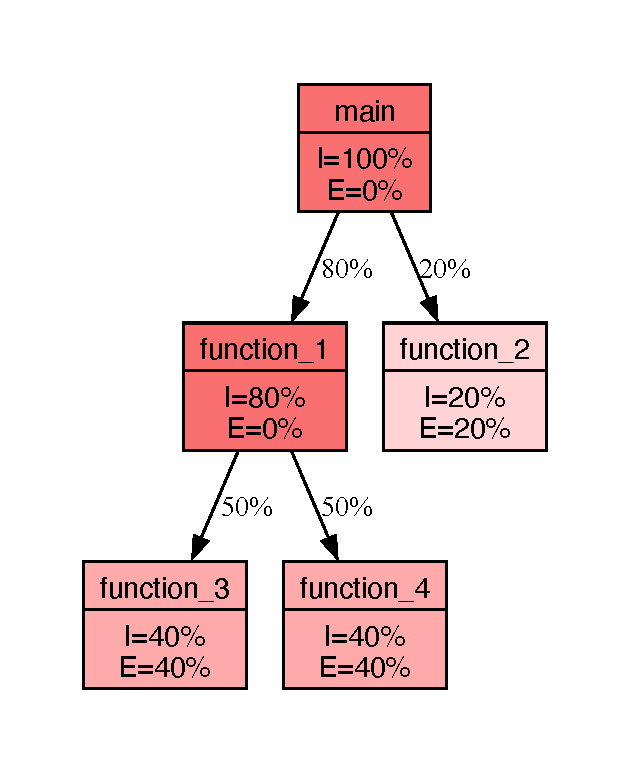
\includegraphics[page=1]{Bilder/pdf/profiler_output_example.pdf}
    \end{center}
    \caption{Beispielausgabe des HANA Profilers}\label{fig:beispielausgabe_hana_profiler}
\end{figure}

% section HANA Profiler (end)
